We carry out in this section the proof of Theorem~\ref{thm:first_moment}.
A direct computation from eq.~\eqref{eq:def_Zkappa} using the linearity of expectation yields:
\begin{equation}
    \label{eq:E_Zr}
    \EE Z_\kappa = \sum_{\eps \in \{\pm 1\}^n} \bbP\left[\left\|\sum_{i=1}^n \eps_i \bW_i\right\|_{\op} \leq \kappa \sqrt{n}\right] = 2^n \, \bbP[\|\bW\|_\op \leq \kappa],
\end{equation}
where $\bW \sim \GOE(d)$.
The main result we prove is the following.
\begin{proposition}[Left large deviations for the operator norm of a $\GOE(d)$ matrix]
    \label{prop:ldp_Wop}
    Let $\bW~\sim~\GOE(d)$. For any $\kappa > 0$:
    \begin{equation}
        \label{eq:ldp_Wop}
        \lim_{d \to \infty} \frac{1}{d^2} \log \bbP[\|\bW\|_\op \leq \kappa]
        = 
        \begin{dcases}
            \frac{\kappa^4}{128} - \frac{\kappa^2}{8} + \frac{1}{2} \log \frac{\kappa}{2} + \frac{3}{8} &\textrm{ if } \kappa \leq 2, \\
            0 &\textrm{ otherwise.} 
        \end{dcases}
    \end{equation}
\end{proposition}
\noindent
Using Proposition~\ref{prop:ldp_Wop} in eq.~\eqref{eq:E_Zr} (recall that $n/d^2 \to \tau$) yields eq.~\eqref{eq:limit_logEZ}.
The second result of Theorem~\ref{thm:first_moment} is a direct consequence of Markov's inequality combined with eq.~\eqref{eq:limit_logEZ}.
Notice that Markov's inequality even shows that $\bbP[Z_\kappa > 0]$ goes to zero exponentially fast in $d^2$ for $\tau < \tau_1(\kappa)$.

\myskip 
In the remainder of Section~\ref{sec:1st_moment}, we focus on proving Proposition~\ref{prop:ldp_Wop}.
We note first that for $\kappa > 2$ we have $\log \bbP[\|\bW\|_\op \leq \kappa] = \smallO_d(1)$ as a consequence of Theorem~\ref{thm:wigner}. 
We thus focus on the case $\kappa \in (0,2]$ in what follows.

\myskip 
\textbf{Sketch of proof and important related work --}
    The proof of Proposition~\ref{prop:ldp_Wop} builds upon a large deviation principle (with respect to the weak topology) for the empirical spectral measure of a matrix $\bW$ drawn from $\GOE(d)$, \emph{conditioned} on $\|\bW\|_\op \leq \kappa$.
\change{
We study the conditioned law directly, since it is a so-called $\beta$-ensemble (albeit with a singular potential enforcing the spectral norm constraint), 
so that the large deviation analysis follows from the general
results stated in Proposition~\ref{prop:ldp_empirical_measure_conditioned}.
As a direct consequence, we obtain in Corollary~\ref{cor:ldp_Wop_var_principle} the asymptotics of eq.~\eqref{eq:ldp_Wop} as a variational principle over probability measures supported in $[-\kappa,\kappa]$.
We note that one could rely solely on the original large deviations principles for (unconditioned) $\GOE(d)$ matrices proven in~\cite{arous1997large},
however this requires additional care because the set of probability measures supported in $[-\kappa,\kappa]$ has empty interior under the weak topology:
for completeness, we also provide in Appendix~\ref{sec:appendix_ldp} a proof of Corollary~\ref{cor:ldp_Wop_var_principle}, 
that appeared in an earlier version of this work, and which uses only the result of~\cite{arous1997large}.
}
We solve the resulting variational principle using the theory of logarithmic potentials~\citep{saff2013logarithmic} and Tricomi's theorem~\citep{tricomi1985integral}, similarly to the alternative proof of Wigner's semicircle law obtained by \cite{arous1997large} from their large deviations result.
Similar arguments also appeared in the theoretical physics literature~\citep{dean2006large,vivo2007large,dean2008extreme,majumdar2014top}.
We refer to \cite{anderson2010introduction,guionnet2022rare} for more background and open problems in the theory of large deviations for random matrices.

\myskip
\textbf{Remark --}
The following result is a byproduct of our analysis\footnote{
After the present work was made available as a pre-print, the author realized that another proof of Theorem~\ref{thm:lsd_constrained_GOE} had appeared in an unpublished manuscript~\citep{bouali2015constrained}.
}.
\begin{theorem}[Limiting spectral density of a constrained $\GOE(d)$ matrix]\label{thm:lsd_constrained_GOE}
   For $\kappa \in (0,2]$, denote $\bbP_\kappa$ the law of $\bW \sim \GOE(d)$ conditioned on $\|\bW\|_\op \leq \kappa$. 
    If $\bW \sim \bbP_\kappa$, then its empirical spectral density $\mu_\bW$ converges weakly (as $d \to \infty$, and a.s.) to $\mu_\kappa(\rd x) \coloneqq \rho_\kappa(x) \rd x$ given, for $x \in (-\kappa, \kappa)$, by:
    \begin{equation}
        \label{def:rhokappa_1}
        \rho_\kappa(x) \coloneqq \frac{4+\kappa^2-2x^2}{4 \pi \sqrt{\kappa^2 - x^2}}. 
    \end{equation}
    Notice that $\rho_{2}(x) = \sqrt{4 - x^2}/(2\pi)$ is Wigner's semicircle law, see Theorem~\ref{thm:wigner}.
\end{theorem}
\noindent
We illustrate the form of $\rho_\kappa(x)$ in Figure~\ref{fig:rho_kappa}.
Theorem~\ref{thm:lsd_constrained_GOE} is proven in Section~\ref{subsec:proof_lsd_constrained_GOE}.
\begin{figure}[!t]
   \centering
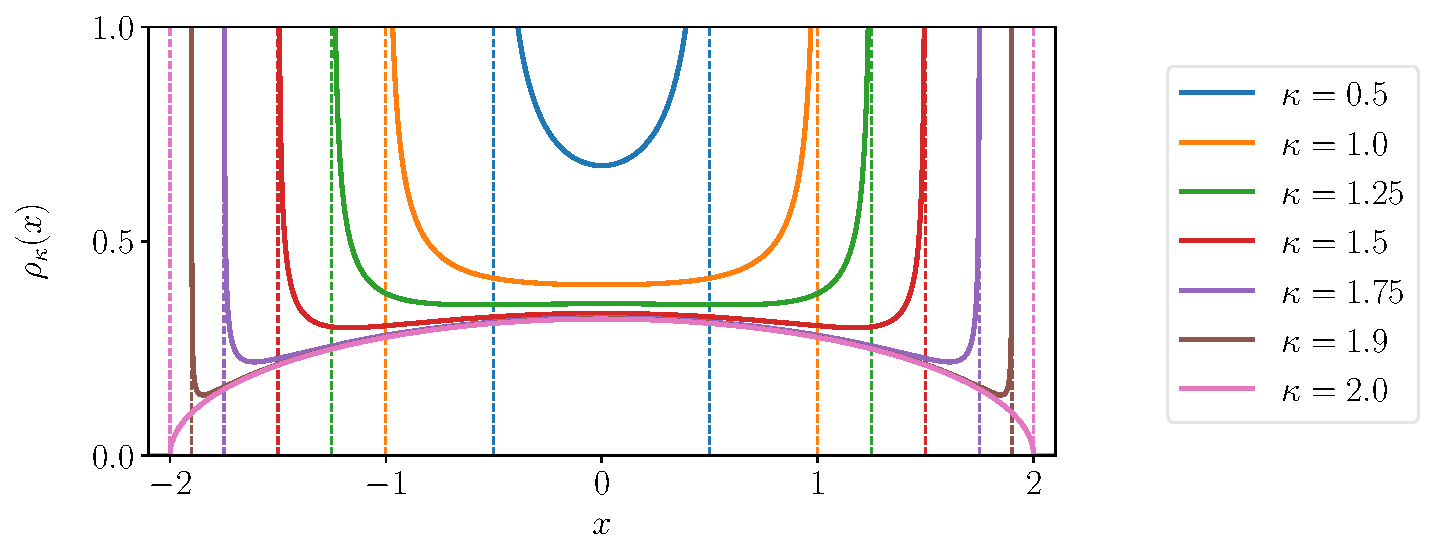
\includegraphics[width=0.9\textwidth]{figures/rho_kappa.pdf}
\caption{$\rho_\kappa(x)$ of eq.~\eqref{def:rhokappa_1} for different values of $\kappa$. For $\kappa = 2$ one recovers the semicircle law.\label{fig:rho_kappa}}
\end{figure}

\myskip
Let us denote
$S_\kappa \coloneqq \{\eps \in \{\pm 1\}^n \, \textrm{s.t.} \, \|\sum_{i=1}^n \eps_i \bW_i\|_{\op} \leq \kappa \sqrt{n} \}$,
so that $Z_\kappa = \# S_\kappa$.
Anticipating our satisfiability results, we note that even if $\bbP[Z_\kappa \geq 1] = 1 - \smallO_d(1)$ as shown in Theorem~\ref{thm:second_moment} for sufficiently large $\tau = n/d^2$, Theorem~\ref{thm:lsd_constrained_GOE} does not ensure that the asymptotic spectrum of $\sum_i \eps_i \bW_i$ (for $\eps \sim \Unif(S_\kappa)$) equals $\rho_\kappa$.
However, one can easily prove that this would be implied e.g.\ by the condition $\EE[Z_\kappa]^2 = (1+\smallO_d(1)) \EE[Z_\kappa]^2$, which is strictly stronger than $\bbP[Z_\kappa \geq 1] = 1 - \smallO_d(1)$.
Unfortunately, the bounds established in Section~\ref{sec:2nd_moment} to prove Theorem~\ref{thm:second_moment} only yield $\EE[Z_\kappa]^2 \leq C \EE[Z_\kappa]^2$ in the satisfiable phase, for a possibly large $C > 1$.
For this reason, we leave the establishment of the limiting spectral density of $\sum_i \eps_i \bW_i$ (for $\eps \sim \Unif(S_\kappa)$) as an open question, 
with $\rho_\kappa$ a natural conjecture.

\subsection{Large deviations results}

Our proof leverages a large deviation principle for the empirical eigenvalue distribution in a large class of matrix models.
Such results were initiated in the mathematics literature by~\cite{arous1997large} in the case of $\GOE(d)$ matrices, and have been then extended, see e.g.~\cite{guionnet2022rare} for a discussion.

\myskip
The space $\mcM_1^+(\bbR)$ of probability measures on $\bbR$ is endowed with its usual weak topology. 
It is metrizable by the Dudley metric~\citep{bogachev2007measure}:
\begin{equation}
    \label{eq:dudley}
    d(\mu, \nu) \coloneqq \left\{\left|\int f \rd \mu - \int f \rd v\right| \, : \, |f(x)| \leq 1 \textrm{ and } |f(x) - f(y)| \leq |x - y|, \, \forall (x, y) \in \bbR^2\right\}.
\end{equation}
Recall that $\Sigma(\mu) \coloneqq \int \mu(\rd x) \mu(\rd y) \log |x-y|$.
The following statement is borrowed from~\cite{fan2015convergence} (variants can be found e.g.\ in~\cite{arous1997large,anderson2010introduction}).
\begin{proposition}[\cite{fan2015convergence}]
    \label{prop:ldp_empirical_measure_conditioned}
    Let $B \subseteq \bbR$ an interval, and $V : B \to \bbR$ a continuous function such that $\lim_{x \to \pm \infty} \frac{V(x)}{2 \log |x|} = +\infty$ (if $B$ is not bounded).
    For $\blambda \in \bbR^d$, let
    \begin{align}\label{eq:coulomb_gas_constraint}
        \mu_{d}^{V,B}(\rd \blambda) \coloneqq \frac{1}{Z_{d}^{V,B}} \prod_{i=1}^d \left(\rd \lambda_i \, \indi\{\lambda_i \in B\} \right) \, e^{-\frac{d}{2} \sum_{i=1}^d V(\lambda_i)} \, \prod_{i < j} |\lambda_i - \lambda_j|,
    \end{align}
    with $Z_d^{V,B}$ a normalization factor, which ensures that $\int \mu_d^{V, B}(\rd \blambda) = 1$.\\
    Denote $\nu_\blambda \coloneqq (1/d) \sum_{i=1}^d \delta_{\lambda_i}$ the empirical measure of $\blambda$.
    Then the law of $\nu_\blambda$ satisfies a large deviation principle, in the scale $d^2$, with good rate function $I_{V,B}(\nu) \coloneqq \mcE_V(\nu) - \inf_{\nu \in \mcM_1^+(B)}[\mcE_V(\nu)]$, where 
    \begin{align}\label{eq:E_V}
        \mcE_V(\nu) \coloneqq - \frac{1}{2} \Sigma(\nu) + \frac{1}{2} \int V(x) \, \nu(\rd x).
    \end{align}
    In particular: 
    \begin{itemize}
        \item[$(i)$] For any $M > 0$, $\{I_{V, B} \leq M\}$ is a compact subset of $\mcM_1^+(B)$.
        \item[$(ii)$]  
        For any open (respectively closed) subset $O \subseteq \mcM_1^+(B)$ (respectively $F \subseteq \mcM_1^+(B)$): 
        \begin{equation*}
            \begin{dcases}
                \liminf_{d\to\infty} \frac{1}{d^2} \log \mu_d^{V,B}[\nu_\blambda \in O] \geq - \inf_{\nu \in O} I_{V,B}(\nu), \\
                \limsup_{d\to\infty} \frac{1}{d^2} \log \mu_d^{V,B}[\nu_\blambda \in F] \leq - \inf_{\nu \in F} I_{V,B}(\nu).
            \end{dcases}
        \end{equation*}
        \item[$(iii)$] 
        \begin{equation*}
            \lim_{d \to \infty} \frac{1}{d^2} \log Z_d^{V,B} = - \inf_{\nu \in \mcM_1^+(B)}[\mcE_V(\nu)].
        \end{equation*}
    \end{itemize}
\end{proposition}
\noindent
 Proposition~\ref{prop:ldp_empirical_measure_conditioned} directly applies to $\bbP_\kappa$, the law of $\bW \sim \GOE(d)$ conditioned on $\|\bW\|_\op \leq \kappa$, 
 with $V(x) = x^2/2$. We obtain from it the following variational formulation for the limit of the left-hand side of eq.~\eqref{eq:ldp_Wop}.
 \begin{corollary}\label{cor:ldp_Wop_var_principle}
    For any $\kappa > 0$, with $\bW \sim \GOE(d)$:
    \begin{equation*}
        \lim_{d \to \infty} \frac{1}{d^2} \log \bbP[\|\bW\|_\op \leq \kappa] = \frac{3}{8} - \inf_{\nu \in \mcM_1^+([-\kappa,\kappa])} \left[-\frac{1}{2} \Sigma(\nu) + \frac{1}{4} \int \nu(\rd x) \, x^2\right].
    \end{equation*}
 \end{corollary}
 \begin{proof}[Proof of Corollary~\ref{cor:ldp_Wop_var_principle}]
    The joint law of the eigenvalues $(\lambda_1, \cdots, \lambda_d)$ of $\bW$ is well-known thanks to the rotation invariance of the law of $\bW$. 
We have (see e.g.\ Theorem~2.5.2 of \cite{anderson2010introduction}):
\begin{align}\label{eq:joint_law_evalues}
    \bbP[\|\bW\|_\op \leq \kappa] &= \frac{\int_{[-\kappa,\kappa]^d} \prod_{i < j} |\lambda_i - \lambda_j| e^{-\frac{d}{4} \sum_{i=1}^d \lambda_i^2} \prod_{i=1}^d \rd \lambda_i}{\int_{\bbR^d} \prod_{i < j} |\lambda_i - \lambda_j| e^{-\frac{d}{4} \sum_{i=1}^d \lambda_i^2} \prod_{i=1}^d \rd \lambda_i}.
\end{align}
The denominator (or partition function) can be computed from Selberg's integrals~\citep{mehta2014random}.
Its limit is given by
\begin{align}\label{eq:part_function_selberg}
    \lim_{d \to \infty} \frac{1}{d^2} \log \int_{\bbR^d} \prod_{i < j} |\lambda_i - \lambda_j| e^{-\frac{d}{4} \sum_{i=1}^d \lambda_i^2} \prod_{i=1}^d \rd \lambda_i 
    &= - \frac{3}{8}.
\end{align}
The result follows then from Proposition~\ref{prop:ldp_empirical_measure_conditioned}-$(iii)$.
 \end{proof}

 \myskip
 \textbf{Alternative proof --}
 For reasons of completeness, and as a first version of this manuscript contained it, we detail in Appendix~\ref{sec:appendix_ldp} a proof of Corollary~\ref{cor:ldp_Wop_var_principle} 
 that does not rely on Proposition~\ref{prop:ldp_empirical_measure_conditioned}, but only on its particular case $B = \bbR$ and $V(x) = x^2/2$, i.e.\ when $\mu_{d}^{V,B}$ is the joint law of the eigenvalues of a $\GOE(d)$ matrix.
 This setting was tackled in the seminal work of~\cite{arous1997large}.
 
 \subsection{Solving the variational principle: proof of Proposition~\ref{prop:ldp_Wop}}\label{subsec:var_principle_1st_mom}

 For $\mu \in \mcM_1^+(\bbR)$, let 
\begin{equation}\label{eq:def_I}
    I(\mu) \coloneqq -\frac{1}{2} \Sigma(\mu) + \frac{1}{4} \int \mu(\rd x) \, x^2 - \frac{3}{8}.
\end{equation}
 We establish here the following equation, for $\kappa \leq 2$: 
 \begin{align}\label{eq:to_prove_var_1st_mom}
    E_\kappa \coloneqq \inf_{\mu \in \mcM_1^+([-\kappa, \kappa])} I(\mu) = 
    - \frac{\kappa^4}{128} + \frac{\kappa^2}{8} - \frac{1}{2} \log \frac{\kappa}{2} - \frac{3}{8}.
 \end{align}
 Combining eq.~\eqref{eq:to_prove_var_1st_mom} with Corollary~\ref{cor:ldp_Wop_var_principle} yields then Proposition~\ref{prop:ldp_Wop}.

 \myskip 
In order to characterize the minimizer of $I(\mu)$ for $\mu \in \mcM_1^+([-\kappa,\kappa])$, we
rely on classical results of logarithmic potential theory, such as Theorem~1.3 of Chapter~I of \cite{saff2013logarithmic}, see also \cite{mhaskar1985does} and Theorem~2.4 of \cite{arous1997large}.
In our context, the ``admissible weight function'' of~\cite{saff2013logarithmic} reads
\begin{equation*}
    w(x) = \exp\{-x^2/4\} \indi\{|x| \leq \kappa\}.
\end{equation*}
Adapting the results of the aforementioned literature to our notations, we obtain the following theorem.
\begin{theorem}[\cite{saff2013logarithmic}]
    \label{thm:properties_inf_I}
    Let $\kappa > 0$ and
    $E_\kappa \coloneqq \inf_{\mu \in \mcM_1^+([-\kappa,\kappa])} I(\mu)$. Then
    \begin{itemize}
        \item[$(i)$] $E_\kappa < \infty$.
        \item[$(ii)$] There exists a unique $\mu_\kappa^\star \in \mcM_1^+([-\kappa,\kappa])$ such that $I(\mu_\kappa^\star) = E_\kappa$.
        \item[$(iii)$] $\mu_\kappa^\star$ is the unique measure in $\mcM_1^+([-\kappa,\kappa])$ such that for $\mu_\kappa^\star$-almost all $x$: 
        \begin{equation*}
            \int \mu_\kappa^\star(\rd y) \, \log |x - y| = \frac{x^2}{4} + \frac{1}{4} \int \mu_\kappa^\star(\rd y) \, y^2 - \frac{3}{4} - 2 E_\kappa.
        \end{equation*}
    \end{itemize} 
\end{theorem}
\noindent
One can further show that this theorem allows to prove that a candidate measure is the optimal one without computing $E_\kappa$.
\begin{lemma}\label{lemma:log_pot_mukappa}
    For $\kappa \in (0,2]$, assume that $\mu \in \mcM_1^+([-\kappa,\kappa])$ and $C \in \bbR$ are such that for all $x \in (-\kappa,\kappa)$:
    \begin{equation}\label{eq:log_pot_mukappa_hyp}
        \int \mu(\rd y) \, \log |x - y| = \frac{x^2}{4} + C.
    \end{equation}
    Then $\mu = \mu_\kappa^\star$.
\end{lemma}
\noindent
Note that Lemma~\ref{lemma:log_pot_mukappa} can also be seen as a consequence of Theorem~3.3 of Chapter~I of \cite{saff2013logarithmic}. 
We give here a short proof for the sake of completeness.
\begin{proof}[Proof of Lemma~\ref{lemma:log_pot_mukappa} --]
    For any $\sigma, \nu$ real signed measures, we have (recall eq.~\eqref{eq:def_I}) 
    \begin{equation*}
        I(\sigma + \nu) - I(\sigma) = -\frac{1}{2} \Sigma(\nu) + \int \nu(\rd x) \left[\frac{x^2}{4} - \int \sigma(\rd y) \log |x - y|\right]. 
    \end{equation*}
    Applying this formula to $\sigma = \mu$ and $\nu = \mu_\kappa^\star - \mu$, we reach:
    \begin{align*}
        I(\mu_\kappa^\star) - I(\mu) &= -\frac{1}{2} \Sigma(\mu_\kappa^\star - \mu) + \int (\mu_\kappa^\star - \mu)(\rd x) \left[\frac{x^2}{4} - \int \mu(\rd y) \log |x - y|\right], \\ 
         &\aeq -\frac{1}{2} \Sigma(\mu_\kappa^\star - \mu), \\ 
         &\bgeq 0.
    \end{align*}
    We used eq.~\eqref{eq:log_pot_mukappa_hyp} in $(\rm a)$ and the fact that $\mu_\kappa^\star$ has no atom since $I(\mu_\kappa^\star) < \infty$~\citep{arous1997large}, so we can restrict the integral 
    to $x \in (-\kappa,\kappa)$.
    In $(\rm b)$ we used the following classical property of the non-commutative entropy $\Sigma(\mu)$, 
    which can be found e.g.\ as Proposition~II.2.2 in \cite{faraut2014logarithmic}.
    \begin{lemma}\label{lemma:nonc_entropy_pos}
        Let $\mu$ be a signed measure on $\bbR$ with compact support, and such that $\int_\bbR \mu(\rd x) = 0$. 
        Let $\hat{\mu}(t) \coloneqq \int \mu(\rd x) \, e^{i t x}$ be the \change{characteristic function} of $\mu$.
        Then 
        \begin{equation*}
            \Sigma(\mu) \coloneqq \int \mu(\rd x) \mu(\rd y) \log |x - y| = - \int_0^\infty \frac{|\hat{\mu}(t)|^2}{t} \rd t.
        \end{equation*}
        In particular, $\Sigma(\mu) \leq 0$.
    \end{lemma}
    \noindent
    This shows that $I(\mu) \leq I(\mu_\kappa^\star) = \inf_{\mu \in \mcM_1^+([-\kappa,\kappa])} I(\mu)$. By $(ii)$ of Theorem~\ref{thm:properties_inf_I}, $\mu = \mu_\kappa^\star$.
\end{proof}
\noindent
Thanks to Lemma~\ref{lemma:log_pot_mukappa}, we can give an exact formula for $\mu_\kappa^\star$ by exhibiting a candidate measure satisfying eq.~\eqref{eq:log_pot_mukappa_hyp}, which in turns implies the exact formula~\eqref{eq:to_prove_var_1st_mom} for $E_\kappa$.
\begin{proposition}
    \label{prop:mukappa_value}
    Let $\kappa \in (0,2]$.
    Recall that $E_\kappa = \inf_{\mu \in \mcM_1^+([-\kappa,\kappa])} I(\mu)$ is reached in a unique measure $\mu_\kappa^\star$.
    Let $\mu_\kappa(\rd x) \coloneqq \rho_\kappa(x) \rd x$ be given, for $x \in (-\kappa,\kappa)$, by:
    \begin{equation}\label{eq:def_rhokappa}
        \rho_\kappa(x) \coloneqq \frac{4+\kappa^2-2x^2}{4 \pi \sqrt{\kappa^2 - x^2}}. 
    \end{equation}
    Then $\mu_\kappa = \mu_\kappa^\star$, and we have eq.~\eqref{eq:to_prove_var_1st_mom}:
    \begin{equation*}
        E_\kappa = I(\mu_\kappa^\star) = - \frac{\kappa^4}{128} + \frac{\kappa^2}{8} - \frac{1}{2} \log \frac{\kappa}{2} - \frac{3}{8}.
    \end{equation*}
\end{proposition}
\noindent
\begin{proof}[Proof of Proposition~\ref{prop:mukappa_value}] 
    By Lemma~\ref{lemma:log_pot_mukappa}, to show that $\mu_\kappa = \mu_\kappa^\star$ it is enough to show that eq.~\eqref{eq:log_pot_mukappa_hyp} 
    holds for $\mu_\kappa$. 
    Since $U(x) \coloneqq \int \mu_\kappa(\rd y) \log |x-y|$ satisfies (in the sense of distributions)
    \begin{equation*}
        U'(x) = \textrm{P.V.} \int \frac{\rho_\kappa(y)}{x-y} \rd y,
    \end{equation*}
    it is enough to check for any $x \in (-\kappa,\kappa)$:
    \begin{equation}\label{eq:to_show_rhokappa}
        \textrm{P.V.}\int_{-r}^r \frac{\rho_\kappa(y)}{x-y} \rd y = \frac{x}{2}, 
    \end{equation}
    where $\textrm{P.V.}$ refers to the principal value. 
    Notice that
    \begin{equation*}
        \textrm{P.V.}\int_{-r}^r \frac{\rho_\kappa(y)}{x-y} \rd y = \lim_{\eps \downarrow 0} \Re\left\{\int_{-r}^r \frac{\rho_\kappa(y)}{x+i\eps-y} \rd y\right\}.
    \end{equation*}
    We compute $G_\kappa(z) \coloneqq \int_{-r}^r \rho_\kappa(y)/(z-y) \rd y$ for all $z$ such that $\Im(z) > 0$.
    Changing variables to $y = \kappa \cos \theta$, and then to $\zeta = e^{i \theta}$, we have:
    \begin{align*}
        G_\kappa(z) &= \frac{1}{4\pi} \int_0^\pi \frac{4+\kappa^2 -2 \kappa^2 \cos^2 \theta}{z - \kappa \cos \theta} \, \rd \theta, \\ 
        &= \frac{1}{8\pi} \int_{-\pi}^\pi \frac{4+\kappa^2 -2 \kappa^2 \cos^2 \theta}{z - \kappa \cos \theta} \, \rd \theta, \\
        &= \frac{1}{8 i\pi} \oint_{|\zeta| = 1} \frac{\kappa^2 \zeta^4 - 8 \zeta^2 + \kappa^2}{\zeta^2(\kappa\zeta^2 -2 \zeta z + \kappa)} \rd \zeta.
    \end{align*}
    The denominator has three poles: $\{0, \zeta_-, \zeta_+\}$, where $\zeta_{\pm} \coloneqq (z \pm \sqrt{z^2-\kappa^2})/\kappa$ (we choose the branch of the square root such that $\Im[\sqrt{w}] \geq 0$ for all $w \in \bbC$).
    Since $\Im(z) > 0$, it is easy to show that $|\zeta_-| < 1 < |\zeta_+|$.
    We then apply the residue theorem and find:
    \begin{equation}\label{G_rhokappa}
        G_\kappa(z) = \frac{z}{2} + \frac{4+\kappa^2-2z^2}{4\sqrt{z^2-\kappa^2}}.
    \end{equation}
    Taking $\lim_{\eps \to 0} \Re[G_\kappa(x+i \eps)]$ for $|x| < \kappa$ yields eq.~\eqref{eq:to_show_rhokappa}, and thus $\mu_\kappa = \mu_\kappa^\star$. 
    It remains to compute $E_\kappa = I(\mu_\kappa^\star)$.
    One can use the same arguments as above (based on the residue theorem) to show 
    \begin{equation}
        \label{eq:int_mukappa_x2}
        \int \mu_\kappa^\star(\rd x) \, x^2 = \frac{\kappa^2(8-\kappa^2)}{16}. 
    \end{equation}
    By $(iii)$ of Theorem~\ref{thm:properties_inf_I} and Lemma~\ref{lemma:log_pot_mukappa},
    we then have for all $x \in (-\kappa,\kappa)$:
    \begin{equation}
        \label{eq:Ekappa_1}
        E_\kappa = \frac{\kappa^2(8-\kappa^2)}{128} - \frac{3}{8} + \frac{x^2}{8} - \frac{1}{2} \int_{-\kappa}^\kappa \rho_\kappa(y) \, \log |x-y| \, \rd y.  
    \end{equation}
    Notice that eq.~\eqref{G_rhokappa} is valid for all $z$ with $\Im(z) > 0$. In particular, we reach from it, that for all $x \geq 0$:
    \begin{equation*}
        \textrm{P.V.}\int_{-r}^r \frac{\rho_\kappa(y)}{x-y} \rd y =
        \begin{dcases}
            \frac{x}{2} & \textrm{ if } x < \kappa, \\ 
            \frac{x}{2} + \frac{4+\kappa^2-2x^2}{4\sqrt{x^2-\kappa^2}} & \textrm{ if } x > \kappa.
        \end{dcases}
    \end{equation*}
    Since this is an integrable function, we have
    \begin{equation*}
        \int_{-\kappa}^\kappa \rho_\kappa(y) \, \log |x-y| \, \rd y =
        \begin{dcases}
            \frac{x^2}{4} + C & \textrm{ if } x \leq \kappa, \\ 
            \frac{x^2}{4} + C - \frac{x\sqrt{x^2-\kappa^2}}{4} - \log\left(\frac{x-\sqrt{x^2-\kappa^2}}{\kappa}\right) & \textrm{ if } x > \kappa.
        \end{dcases}
    \end{equation*}
    Using that $\int_{-\kappa}^\kappa \rho_\kappa(y) \log |x-y| \rd y - \log x \to 0$ as $x \to \infty$ yields $C = \log(\kappa/2) - \kappa^2/8$.
    Eq.~\eqref{eq:Ekappa_1} becomes:
    \begin{align*}
        E_\kappa = I(\mu_\kappa^\star) &= \frac{\kappa^2(8-\kappa^2)}{128} - \frac{3}{8}  - \frac{1}{2} \left[\log \frac{\kappa}{2} - \frac{\kappa^2}{8}\right], \\ 
        &= - \frac{\kappa^4}{128} + \frac{\kappa^2}{8} - \frac{1}{2} \log \frac{\kappa}{2} - \frac{3}{8},
    \end{align*}
    which ends the proof.
\end{proof}
\myskip
\textbf{Remark: predicting the form of $\rho_\kappa$ --} In order to predict the density $\rho_\kappa$ given by eq.~\eqref{eq:def_rhokappa}, 
we used an argument based on a heuristic application of Tricomi's theorem~\citep{tricomi1985integral}, which states that if eq.~\eqref{eq:to_show_rhokappa} is satisfied 
and $\rho_\kappa$ is supported on $[-\kappa,\kappa]$, then 
\begin{equation}\label{eq:tricomi}
    \rho_\kappa(x) = \frac{1}{\pi \sqrt{\kappa^2-x^2}}\left[C - \frac{1}{\pi} \textrm{P.V.} \int_{-\kappa}^\kappa \frac{\sqrt{\kappa^2-y^2}}{x-y} \times \left(\frac{y}{2}\right) \rd y\right],
\end{equation}
for some constant $C$ chosen to ensure $\int_{-\kappa}^\kappa \rho_\kappa(x) \rd x = 1$.
A careful evaluation of eq.~\eqref{eq:tricomi} based on the residue theorem yields eq.~\eqref{eq:def_rhokappa}.



\subsection{Limiting spectral distribution of a norm-constrained Gaussian matrix}\label{subsec:proof_lsd_constrained_GOE}

Theorem~\ref{thm:lsd_constrained_GOE} follows as a direct consequence of Proposition~\ref{prop:ldp_empirical_measure_conditioned} and Proposition~\ref{prop:mukappa_value}.
Indeed, let $\bbP_\kappa$ be the law of $\bW \sim \GOE(d)$ conditioned on $\|\bW\|_\op \leq \kappa$, and denote $\mu_\bW$ the empirical spectral distribution of $\bW$.
Then for any $\delta > 0$, if $B(\mu_\kappa^\star,\delta) \subseteq \mcM_1^+([-\kappa,\kappa])$ is the open ball of radius $\delta$ centered in $\mu_\kappa^\star$ for the distance of eq.~\eqref{eq:dudley}, 
\begin{align*}
    \limsup_{d \to \infty} \frac{1}{d^2} \log \bbP_\kappa[\mu_\bW \notin B(\mu_\kappa^\star, \delta)] \leq - \inf_{\mu \in B(\mu_\kappa^\star, \delta)^c} [J_\kappa(\mu)],
\end{align*}
with 
\begin{align*}
    J_\kappa(\mu) \coloneqq I(\mu) - I(\mu_\kappa^\star),
\end{align*}
for $I$ given in eq.~\eqref{eq:def_I}.
Since $J_\kappa$ is a good rate function (see Proposition~\ref{prop:ldp_empirical_measure_conditioned}) and has a unique minimizer (cf.\ $(ii)$ of Theorem~\ref{thm:properties_inf_I}), 
$\inf_{\mu \in B(\mu_\kappa^\star, \delta)^c} [J_\kappa(\mu)] > 0$. Therefore, by the Borel-Cantelli lemma,
\begin{align*}
    \bbP[\limsup_{d \to \infty} d(\mu_\bW, \mu_\kappa^\star) \leq \delta] = 1,
\end{align*}
which ends the proof by taking the limit $\delta \to 0$.
$\qed$